\newpage
\subsubsection{Swellpro Fisherman FD1}
\begin{wrapfigure}{r}{0.3\textwidth}
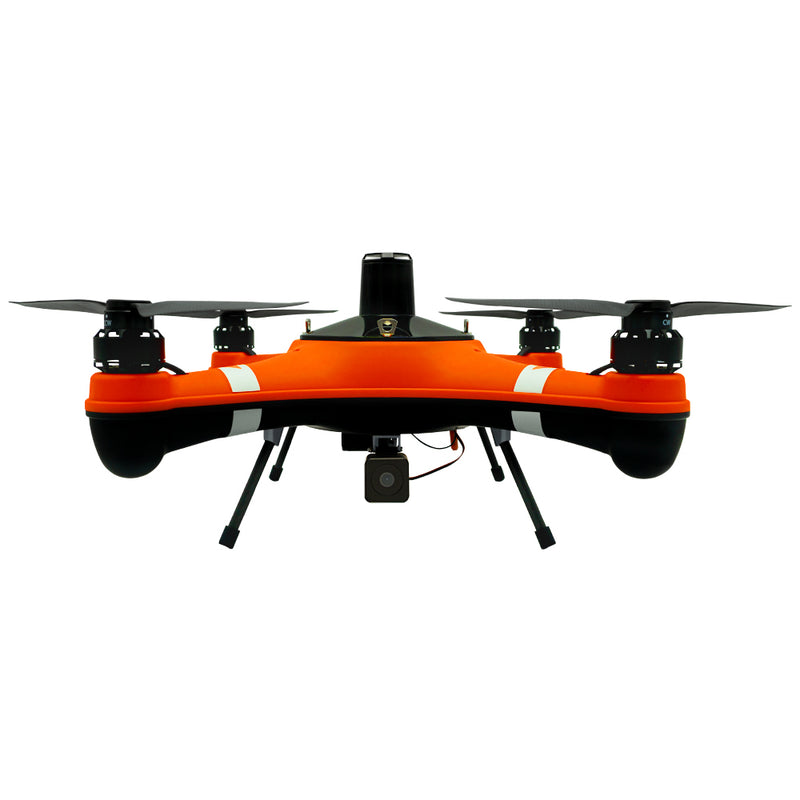
\includegraphics[width=1\linewidth]{uav/models/11_fishermanfd1.png}
\caption{Fisherman FD1}
\end{wrapfigure}
The Fisherman FD1 \cite{fishermanfd1} is Swellpro's economical offering based on their previous flagship. It is also fully designed to be used in the water.

\paragraph{Payload capacity}\mbox{Score: 1.5} \\
The payload capacity of the Fisherman FD1 is 2kg, well above the minimum requirement.

\paragraph{Mounting clearance}\mbox{Score: 1.1} \\
The Fisherman FD1 is a medium compact drone and therefore doesn't have a lot of clearance for sensors. One could create their own platform beneath the drone, utilizing the four feet.

\paragraph{Navigation/Routing}\mbox{Score: 0.5} \\
While the Fisherman FD1 is based off of the SplashDrone 3+ that has an app that allows waypoints, it is not clear if this revised version can use that app as well. One might need to acquire a remote from the SplashDrone 3+ for the app to work.
As an alternative, one could hack into the internals of the drone with relative ease and use an open source flight system like ArduPilot.

\paragraph{Flight time}\mbox{Score: 1.5} \\
The flight time of the SplashDrone 4 is 30 minutes, well over the minimum required flight time.

\paragraph{Range}\mbox{Score: 1.2} \\
The maximum radio range is 1.6km, passing the minimum required range. This includes image transmission.

\paragraph{Waterproof}\mbox{Score: 1.5} \\
The drone is IP67 waterproof, meaning the drone is dust-tight and can immerse up to 1 meter in water. This is well over the minimum required IP rating.

\paragraph{Landing in water}\mbox{Score: 1.5} \\
The drone is designed to land and take off in the water.

\paragraph{Maneuverability}\mbox{Score: 1.1} \\
The drone can fly horizontally 10m/s with the GPS being the limiting factor.

\paragraph{Total score:}\mbox{3.7} \\
The Fisherman FD1 looks like a capable budget-friendly alternative to the SplashDrone 4, but the compatibility of the waypoint app needs to be figured out.

